%% Supporting Information for the Macromolecules manuscript (main.tex). Written 2026-10-27 from the methods and
%% extended results of the 2026-10-21 draft, the ontology refinement plan (Part C), the app latency plan and the
%% confirmation plan. Section numbers are cited literally from main.tex (Section S1 ... S16): keep the order.
\PassOptionsToPackage{hyphens}{url}
\documentclass[journal=mamobx,manuscript=suppinfo]{achemso}

\usepackage{graphicx}
\usepackage{booktabs}
\usepackage{siunitx}
\usepackage{xcolor}
\usepackage{url}
\usepackage{listings}

%% Single-spaced throughout, as main.tex; the class double-spaces manuscripts.
\AtBeginDocument{\singlespacing}

\SectionNumbersOn
\renewcommand{\thesection}{S\arabic{section}}
\renewcommand{\thefigure}{S\arabic{figure}}
\renewcommand{\thetable}{S\arabic{table}}

\newcommand{\tbd}[1]{\textcolor{red}{[#1]}}
\newcommand{\code}[1]{\texttt{#1}}
\newcommand{\ident}[1]{\path{#1}}

%% Room in the contents for two-digit section numbers (S10-S16).
\makeatletter
\renewcommand\@pnumwidth{2em}\renewcommand\@tocrmarg{3em}
\renewcommand*\l@section{\@dottedtocline{1}{0em}{2.6em}}
\renewcommand*\l@subsection{\@dottedtocline{2}{2.6em}{3.4em}}
\makeatother

\lstset{basicstyle=\ttfamily\scriptsize, breaklines=true, columns=fullflexible, keepspaces=true,
  frame=single, rulecolor=\color{black!30}, xleftmargin=0.5em, xrightmargin=0.5em}

\author{Brett M. Savoie}
\email{bsavoie2@nd.edu}
\affiliation[University of Notre Dame]
{Department of Chemical and Biomolecular Engineering, University of Notre Dame, Notre Dame, Indiana 46556, United States}

\title{Open Ontology of Polymer Chemistry: Accumulation and Self-Improving Memory Mechanisms for Polymer Research}

\begin{document}

\maketitle

\tableofcontents

%% ---------------------------------------------------------------------------------------------
\section{Seed Ontology and Data Model}
\label{si:seed}

The seed was imported from a pinned snapshot of WOP, a public reference for polymer families and established polymer materials in which every populated article section cites open sources.\cite{WOP2026Wiki}
The snapshot provides 274 polymer concepts with stable identifiers, 245 MDL V3000 structures, 16,925 claims, 3,785 evidence records, 2,349 documents, 144 taxonomy facets, 275 processes, and 3,562 article sections, or 27,559 records in all (Table~\ref{tbl:counts}).
The importer is one-way.
It preserves WOP identifiers, article-local evidence, classification axes, synthesis routes, and structure strings byte for byte, and it performs no new literature research.
Scientific assertions are stored as claim records with a subject, predicate, object, context, and evidence, so that two differently qualified assertions about the same pair of entities remain separate records.
Imported claims keep the status \emph{seed}; importing a source-backed draft is not a review, and nothing in the present study promotes a seed claim.
Canonical records are JSON-LD.
SQLite with full-text search, RDF N-Triples, and browsable pages are projections derived from them, and every release is named by a hash of its canonical content.
Provenance fields map to the W3C PROV ontology.\cite{Lebo2013PROVO}

The knowledge layer is a separate store.
A finding is one source-qualified value.
It comprises a one-sentence statement, the material as specifically as the source identifies it, the property by its full name and abbreviation, the value as reported with its unit, and the conditions as the source states them (specimen, processing history, method, and test conditions).
It also records the source's title, URL, and DOI, an exact locator (section, table, figure, or page), and a verbatim excerpt of at most about 25 words that shows the value together with its label.
A source note records each source a session read, including sources that lacked what was sought or could not be opened, with the URL at which it was read.
Findings carry one of four statuses.
\emph{Reviewed} findings were supported by a reviewer session, \emph{Added} findings were saved on the researcher's judgement, \emph{Needs checking} findings await review or could not be confirmed by their reviewer, and \emph{Rejected} findings were judged unsupported.
Rejected findings are never returned by search but are kept with the reviewer's reason.
Excerpts are kept privately as provenance for reviewers; the released knowledge snapshot carries every other field.

\begin{table}
  \caption{Seed and Knowledge Base at the Freeze}
  \label{tbl:counts}
  \begin{tabular}{lr}
    \toprule
    item & count \\
    \midrule
    \multicolumn{2}{l}{\emph{seed release (WOP)}} \\
    polymer concepts & 274 \\
    V3000 structures & 245 \\
    claims & 16,925 \\
    evidence records & 3,785 \\
    documents & 2,349 \\
    records in all & 27,559 \\
    \multicolumn{2}{l}{\emph{knowledge base (KF)}} \\
    completed questions & 1,092 \\
    questions that saved a finding or note & 942 \\
    findings & 8,899 \\
    \quad Reviewed / Added & 5,489 / 3,268 \\
    \quad Needs checking / Rejected & 124 / 18 \\
    source notes & 2,195 \\
    distinct sources (with findings) & 1,679 (951) \\
    polymers with a finding & 157 \\
    reviews (Codex / Claude Code) & 1,830 (1,603 / 227) \\
    \multicolumn{2}{l}{\emph{campaign new tokens (millions)}} \\
    research / review / checks & 49.0 / 13.2 / 2.30 \\
    \bottomrule
  \end{tabular}
  %% Tokens: the 92 answers before the 200-task run have no ledger; the cleanup's reviews (28.8 M) are separate.
\end{table}

%% ---------------------------------------------------------------------------------------------
\section{Polymer Resolution}
\label{si:resolution}

A polymer named in a question or a finding is resolved to a seed identity through the seed's names and aliases, grade designations, trade names recorded in the seed, and family membership.
For example, EVOH44 resolves to ethylene vinyl alcohol copolymer and Ultem to polyetherimide.
Resolution also follows the taxonomy, so a search for high-density polyethylene returns findings filed under the polyethylene family but not those filed under low-density polyethylene.
Three abbreviations name unrelated polymers in the seed (PEI, PFA, and PPO).
A question that uses one of them is returned to its asker for clarification; in the automated runs reported here, which have no asker, the researcher states its reading.
A saved finding is filed under the polymer named by its material or statement when they name exactly one; otherwise it is filed under the polymer named by the question.
A finding that names several polymers, such as a blend, is not filed under the question's polymer.
An ambiguous material label that cannot be settled from the question and source is not saved as written.
It is sent to review instead, and the reviewer writes the material out from the source.

%% ---------------------------------------------------------------------------------------------
\section{Researcher Session}
\label{si:researcher}

Each question is answered by one non-interactive session of a subscription coding agent with read-only file access, live web search, and one additional tool, \code{search\_knowledge} (Section~\ref{si:search}).
All controlled experiments used OpenAI's Codex agent with the model gpt-6.1-sol for research, review, and checking, unless stated otherwise; Anthropic's Claude Code with the model claude-opus-5-5 was used for the cross-engine experiment, for scaffold improvement, for the ontology curator, and for blind scoring.
Every engine call either returns a valid response or fails with a named reason (timeout, crash, rejection, invalid output, interruption, missing sign-in, quota, or rate limit), and transient failures are retried once.
The researcher's instructions are a single prompt, reproduced in Section~\ref{si:prompts}, that is identified by the first 12 hexadecimal characters of the SHA-256 hash of its text.
All controlled experiments and the ontology refinement used the frozen prompt \ident{0b7bb1483235}.
At the standard depth used throughout, a session has a 10~min limit and a budget of about ten web searches and eight sources.
A source is one document, and rereading another part of it does not count against the budget.
The prompt instructs the researcher to search saved knowledge before the web, to cite a saved finding rather than reopen its source, and to treat findings that need checking, together with source notes, as leads to be confirmed.
It also instructs the researcher to prefer open HTML full text over PDF copies and to stop after about two further searches for any one missing detail.

An answer contains three kinds of statement.
A statement of what a source reports carries an inline citation, which is either a finding identifier or a source URL.
The researcher's own reasoning, such as a comparison, a unit conversion, or a judgement that sources disagree or that a value looks mislabelled, begins with ``Interpretation:'' and cites its premises.
Textbook background begins with ``Background:'' and carries no citation.
Conflicting values are reported side by side with their sources, and the reading of the conflict is given as an Interpretation.
A number seen only in a search snippet may not be reported as a result.
Alongside the answer, the session returns its citations, the new findings it read, one note per source read, its limitations, and up to three open questions.
Every value the answer reports from a source the session read must be saved as a finding, one value per finding.
The researcher also saves up to about ten further values from the same passage that describe the same material or a closely related property, because reading them again later would cost another session.
Each finding also records whether its value was read in the text or a table, read off a figure, converted or calculated, or combined from more than one passage.

\subsection{The Released Two-Turn Session}
\label{si:twoturn}

In the frozen code used for every experiment except the confirmation run (Section~\ref{si:confirm}), one session returned the answer, its findings, and its source notes in one structured response.
On Part~A's records for the 60 held-out questions, the researcher on K0 took a median 81~s and produced a median 3,779 output tokens per answer, against 35~s and 851 tokens for the plain session; about 1,550 of those tokens were findings and about 325 source notes, against about 280 for the answer itself.
Input tokens are mostly cached, so output tokens explain the gap, and the deposit is about two thirds of it.
Nothing after the answer delays it: the queue, the database write, source capture, Crossref titles, and review all run after the answer is marked done.

The released code (version 0.13.0, tag \code{study-freeze-4}) therefore splits the session into two turns.
The first turn returns the answer, its citations, limitations, and open questions under the answer instructions (Section~\ref{si:prompts}).
The second turn resumes the same session with the same response schema, tools, and web settings, so that its context is cached, and writes the findings and source notes under the deposit instructions, which carry the deposit rules of the frozen prompt verbatim.
The answer is shown as soon as the first turn ends, and the second turn runs in the background.
The next question to the same engine waits for the previous question's findings, so that a follow-up reads what its predecessor saved.
The two turns are identified together by prompt \ident{86404bf073ce}.
The engine's session state is kept in a private folder for the question and deleted afterward, so saved sessions do not enter the engine's own history.
Because Codex reports usage cumulatively over a resumed session, the second turn's usage is recorded as the difference between the two reports; Claude Code reports each turn separately.

The change was kept only after the fixed parity set of eight questions (Section~\ref{si:improve}) recommended it.
Against a baseline run of the frozen prompt, the two-turn session left quality unchanged (no contradicted statement, 8 of 8 answers complete, 8 results given, and 7 passes), lowered the median new tokens from 39.3k to 34.3k, and lowered the median seconds to the answer from 40.9 to 34.5 (44.2 including the second turn).
Eight questions cannot resolve latency changes of 10 to 20~s, because one or two extra web calls outweigh them; a repeat of the same configuration moved the median seconds to the answer from 34.5 to 40.5.
Output tokens are the steadier measure: the answer turn's mean output fell from 1,751 tokens to about 1,080, a 38\% reduction, and the findings moved after the answer (280 to 1,400 output tokens per parity question, and 1,700 to 5,600 on research-heavy questions on K0).
On real questions on K0, the answer arrived after 34 to 56~s, followed by 34 to 60~s of saving in the background with 97\% of the second turn's input cached.
On the confirmation run's 60 held-out questions, however, answers used about a quarter more new tokens than the frozen code had used on the same questions, while the answer still arrived sooner (Section~\ref{si:confirm}).

%% ---------------------------------------------------------------------------------------------
\section{Deposit and Review}
\label{si:review}

A returned finding is saved only if it has a statement, a source, and a locator or an excerpt; malformed findings are dropped and counted.
A fact is not saved twice.
Two findings are duplicates when they share a source (a DOI and its resolver URL are one source) and the same numbers, and they have either the same statement or the same property, value, unit, and material.
After each answer, every finding whose source has a DOI is filed under the title that Crossref gives for that DOI, so a misspelled title does not reach a later answer.
A value the researcher read directly in the text or a table is Added on the researcher's judgement.
A value read off a figure, converted, or combined is Needs checking until it has been reviewed.
This narrow review policy is that of the frozen code; the waves that built the knowledge base used a review flag set by the researcher instead (Section~\ref{si:build}).

Review begins after the answer has been delivered, so an answer never waits for it.
Before review, the open copy of each cited source is fetched once by plain HTTPS outside the agent and its text is stored privately.
The URL at which the researcher read the source, the source URL, the Europe PMC full text for articles in PubMed Central, and the DOI are tried in that order.
A page that refuses access is left uncaptured, and no access control is circumvented.
One reviewer session then checks the answer's findings that need checking, together with a stable random sample of one in five of its Added findings.
The reviewer is a fresh session of the engine that wrote the answer, with web access but no access to the knowledge store.
The reviewer is given the passages of each source's captured text around the finding's value, locator, and conditions, and it opens the live source for anything those passages do not show.
When a method or condition is at stake, it also reads the methods or experimental section.
It returns \emph{supported}, \emph{unsupported}, or \emph{uncertain} for each finding with a one-sentence reason.
A supported finding becomes Reviewed, and the reviewer quotes the span of the source that shows its value; an unsupported finding becomes Rejected; an uncertain finding becomes Needs checking.
A misspelled or wrong source title counts as unsupported.
A review has a 5~min limit, and a failed review is retried once, on the other engine when it is available.

%% ---------------------------------------------------------------------------------------------
\section{Search and Reuse}
\label{si:search}

The \code{search\_knowledge} tool returns the saved findings most relevant to a query, followed by up to three source notes.
A query is matched against a full-text index (SQLite FTS5) of each finding's statement, material, property, conditions, source title, and excerpt, with each polymer name in the query expanded by its other names in the seed (so that PCL also matches polycaprolactone).
When the query names a polymer, only findings filed under that polymer, its broader families, or its narrower members are kept, ranked by the fraction of the query's other words they contain.
Findings that match only the polymer fill a short result up to ten, and the caller may request between 10 and 25 findings.
Up to 12 further findings saved from the same sources follow.
These are usually the method, specimen, and conditions that accompany a value, so a source that has already been read need not be opened again.
Results are grouped as Reviewed, Added, and Needs checking.
Every call to the tool is recorded with its exact returned payload, so whether a finding was returned to a later session, and whether that session cited it, are observed rather than inferred.
Search reads polymer names (label, canonical name, abbreviations, alternate names, and trade names) and broader and narrower links from the seed; in the frozen code nothing links one source to another, and the seed has no property vocabulary.
The ontology refinement (Section~\ref{si:ontology}) adds both, through two changes that do nothing without overlay data.

%% ---------------------------------------------------------------------------------------------
\section{Building the Knowledge Base}
\label{si:build}

The knowledge base studied here, denoted KF, was built in stages through the loop described above and then frozen (Table~\ref{tbl:counts}).
Development use of the loop before the stages described here had saved about 150 findings; this store, dated 2026-10-01, is denoted K0.
A 200-task observation run then asked 160 distinct questions, four angles on each of 40 polymer topics, together with 40 exact repeats.
A campaign of 800 tasks followed in three waves of 150, 250, and 400 tasks.
Its question bank combined each of 135 polymers (40 from the observation run's topics and 95 new) with a property, a factor, or a comparison group that is chemically sensible for the polymer's class.
The 655 first questions were of five kinds, asking for a property (245), a method (122), the effect of a factor (123), an assessment (82), or a comparison (83).
The remaining 145 tasks asked an earlier question again, either exactly, in other words, or about the same polymer and property from another angle (a sibling).
All tasks were run at the standard depth, and 8\% of campaign answers were sampled for whole-answer checks (Section~\ref{si:checking}).
The researcher's prompt, the model, and the review policy changed between waves (Section~\ref{si:improve}), so the records of the build are analyzed descriptively.

Before the freeze, the store was cleaned once for defects left by waves that ran before the corresponding fix.
Source titles were reconciled with Crossref, missing or unlabelled excerpts were quoted from their sources by reviewer sessions, and findings whose sources a reviewer could not open were reviewed again.
Findings without a polymer identity were assigned one where their material named a single polymer, nine trade names approved by a reviewer session were added to the seed so that findings naming a trade grade are filed under its polymer, and duplicates were merged.
The frozen store contains 8,899 findings (5,489 Reviewed, 3,268 Added, 124 Needs checking, and 18 Rejected) and 2,195 source notes.
It is released as knowledge snapshot \ident{oopc-knowledge-db1fc22ca88a0c0b45b9218b}, made against seed release \ident{oopc-6ad56d8b354d053bcc3cf3a1}.

\subsection{Extended Description of the Knowledge Base}

The 200-task observation run saved about two findings per answer, and each campaign wave about ten, under prompts that were revised between stages.
Because questions, prompts, and models changed together between stages, these records describe how the store was built rather than measure the effect of any one change.
Every campaign question was drawn from the bank of 135 polymers, which is why coverage follows the question bank.
The material-property findings span 125 property classes and 1,389 polymer--property pairs, with mechanical properties and thermal transitions recorded for nearly every polymer class.

The 995 DOI sources known to Crossref have a median publication year of 2020, 62.4\% of the DOI sources are open access by Crossref's indicator, and MDPI (363), Elsevier (142), and Wiley (133) are the largest publishers.
The store's source key drops a URL's query string, so a few documents identified only there are merged; counted separately, there are about 1,685 sources.
The researcher reads what it can open, which favors recent open-access articles and freely posted commercial documents.

Conditions, locators, and excerpts are present for 99.1\%, 100\%, and 99.7\% of findings, a polymer identity for 98.2\%, a numeric value for 92.3\%, and a unit for 83.0\%.
Of the 3,443 Added findings sampled for spot checks during the build, reviewers supported 3,372, could not confirm 60, and rejected 11 (0.3\%).
Of the 1,874 findings flagged for review when saved, 1,819 were Reviewed, 49 remained Needs checking, and 6 were Rejected, and 110 of the 124 findings left Needs checking in KF are cases in which the reviewer could not open the source.
In a double review of 100 findings during the cleanup, every Reviewed finding was confirmed again, but 12 of 28 rejections were overturned, mostly over wording, such as a label that the cited table cell lacks but the paper defines elsewhere.

Of KF's 8,899 findings, 72.7\% were returned by at least one later session's search and 16.7\% were cited by at least one later answer, for 2,320 citations in all.
Saved findings make up 63.2\% of the citations in campaign answers, and a cited finding waited a median of 202 answers between its deposit and its first citation.
The share of campaign first questions citing a saved finding rises from 13\% for a polymer with no earlier campaign question to 18\%, 28\%, 37\%, and 44\% after one, two to three, four to six, and seven or more earlier questions.
Of the 124 findings now marked Needs checking, 16 were cited, all while they were still Added or Reviewed.

%% ---------------------------------------------------------------------------------------------
\section{Prompt Improvement}
\label{si:improve}

The researcher's prompt was revised in two ways.
During the campaign, a maintainer agent session (Claude Code) read each wave's records, including failed checks, rejected findings, and answers, and proposed the smallest change to the prompt or code that addressed the dominant failure.
Each change was tested, compared with the previous prompt on a fixed parity set, and committed with the owner's approval, so the prompt was revised after each of the three waves.
The parity set has eight fixed questions, four covered by saved findings and four new, each answered by the researcher and by a plain web session of the same engine (Section~\ref{si:checking}).
Its comparison is a guardrail rather than a gate.
A prompt holds the guardrail when it has at most one more contradicted statement and one fewer complete answer than the plain session, at least 90\% of unlabelled answer parts cited, and a median token ratio of at most 1.5.

During the campaign, each measure that a prompt change targeted moved after that change, but the changes were made by a maintainer session and confounded with new questions and a new model (main text Figure~4e, left).
The share of findings the researcher flagged for review rose from 22.0\% in the 200-task run to 54.3\% in wave 1 and fell to 8.1\% after the change for wave 2, and the share saved with an empty excerpt fell from 24.5\% to 0.56\%.
Review tokens per research token fell from 0.35 to 0.13 and rose to 0.32 when reviews moved to Codex in wave 3, and the share of answers made without the web rose from none to 16.0\%.

Improvement was then automated in a recursive test of three rounds, each of 100 new tasks through the loop on a growing copy of the store.
After each round, one Claude Code session without web access or tools read the round's records and proposed one edit to the prompt, replacing an exact passage of at most 600 characters with at most 1,000 characters.
The current and proposed prompts answered a fixed development set of 30 questions on the round's snapshot, and both answers to a question were checked on the same day.
The edit was adopted if it produced no more contradicted statements, no fewer complete answers, and no fewer sourced results, at a median paired token ratio of at most 1.10 over at least 27 checked pairs.
Two of the three proposed edits were adopted.
The first prefers open HTML copies of a source and cites the DOI or publisher URL when a mirror was read.
The second accepts a patent example, data sheet, or saved finding as answering a question about ``a published study'' and stops retrying a source that will not open.
The frozen prompt carries both edits, together with one sentence, added after the planted-finding experiment (Section~\ref{si:experiments}), that treats an Added finding whose excerpt does not show its value, or whose value looks implausible, as a lead.
The same improver, development set, and adoption rule revised each restart's prompt independently (Section~\ref{si:restarts}).

%% ---------------------------------------------------------------------------------------------
\section{Answer Checking and Measures}
\label{si:checking}

Answers were judged for source support by an independent checker, a fresh Codex session that does not share the researcher's context.
The checker is an LLM judge\cite{Zheng2023Judging} applied to claim verification against cited sources,\cite{Wadden2020SciFact} and its verdicts are treated as measurements with their own noise rather than as ground truth.
The checker is given the question, the answer, each cited source with the passages of its captured text around the values the answer gives, the review status of each cited finding, and the session's record of its knowledge searches and web actions.
It classifies every substantive statement by kind and judges it by that kind's rule.
A source fact is checked at its cited location for material scope, conditions, units, and bibliographic detail; a source that cannot be read and has no captured text makes the statement uncertain rather than contradicted.
An Interpretation is supported when its cited premises hold and its reasoning is sound, and Background is supported when it is correct general polymer science.
A claim about a finding's status, or about what the session's searches returned, is judged against the supplied records.
The checker adds one completeness statement, which is unsupported only when the main requested result is missing, and it states separately whether the answer gave the main result from a cited source or saved finding.
An honest report that the result was not found can therefore be complete without giving a result.
The checker judges source support, not correctness, and no human graded the answers.

Quality is reported first through contradicted statements (statements unsupported for any reason other than source access), complete answers, and sourced results, three measures that do not depend on whether a source opened on the day of the check.
Passes, which require every statement supported and a complete answer, and statements left uncertain for source access are reported second, because checking the same answers a second time moved passes by up to two or three in 20 while leaving contradicted statements almost unchanged.
Cost is measured as new tokens, the uncached input tokens plus output tokens recorded for the session, together with web calls and wall-clock time.
Reuse is measured as the number of answers that cite a saved finding and the number answered without a web call.

The comparison arm P is a plain session of the same engine with web search only and a short instruction to answer, cite each source by URL, keep material, specimen, method, and test conditions explicit, and state limitations.
Every experiment follows the same like-for-like protocol.
The arms of a question are answered in turn, starting at a rotating arm, and all of the question's answers are then checked one after another by the same checker engine on the same day.
Researcher arms answer on copies of their stores and save nothing.

%% ---------------------------------------------------------------------------------------------
\section{Controlled Experiments on the Frozen Knowledge Base}
\label{si:experiments}

All controlled experiments ran from one frozen code revision (tag \code{study-freeze-2}), prompt, seed release, and knowledge base, and each experiment's predictions were written and committed before its first answer.
The main experiments use 60 held-out questions, never asked before, in three strata of 20 at standard depth.
A near question takes the polymer and property of a campaign question that saved at least three findings and asks about them from the other angle (a property question becomes a method question, or the reverse).
A mid question asks about a polymer that had been asked about at least three times, for a property of its class never asked for it.
A far question asks about a polymer with no finding naming it, its family, or its members.

Stores of intermediate size were made by cutting KF at the end of the 200-task run and of campaign waves 1 and 2 (KF200, KF1, and KF2, with 532, 2,170, and 5,021 findings).
Records made after a cut are dropped, a finding reviewed after the cut returns to its state at the cut, and merges made after the cut are undone.
Because the six duplicate merges of the cleanup are undone, each cut holds six more findings than KF credits to that stage (526, 2,164, and 5,015; main text Figure~3a).
The same cut at 2026-10-02 reproduces the finding and note identifiers of K0.

\emph{Memory and scaling (A2).}
The 60 held-out questions were answered by P and by the researcher on K0, KF200, KF1, KF2, and KF, and by the researcher with web search disabled on KF1 and KF (MF1 and MF), with three replicates, for 1,440 answers.

\emph{Resampled stores (A3).}
To separate the size of a store from its coverage of a question's topic, 20 further stores were built by filtering KF's findings and notes by the question that saved them.
They comprise nested random subsets of 100, 200, 400, and 800 of the 953 questions that saved a finding or a note, with five random orderings, and no new research was performed to build them.
The 60 held-out questions were answered on each, with K0 and KF answered alongside as same-day anchors (1,320 answers).

\emph{Similarity ladder (A4).}
Thirty campaign first questions were drawn as parents.
Each asks about a single polymer with at least three findings in KF, was never revisited during the campaign, and has a polymer--property pair that no other first question asked.
Each parent was asked again exactly, in other words, and as a sibling, and the 90 questions were answered on K0 and KF with two replicates (360 answers).

\emph{Case studies and planted findings (A5).}
Four case studies were each run five times with the researcher on KF beside P.
The first asks for glass transition temperatures, and their dependence on method and conditions, for three polymers whose saved values span DSC and DMA.
The second asks why published oxygen permeabilities differ for films of poly(vinylidene chloride) (PVDC), poly(3-hydroxybutyrate-\emph{co}-3-hydroxyvalerate) (PHBV), and poly(propylene carbonate) (PPC).
The third asks for two rankings of polymers by oxygen permeability and is also answered by the researcher on an empty store.
The fourth asks for three properties not expected to be reported in open sources, first through the loop and then again in other words.
Case-specific counts, such as values reported with their method or conditions, were scored from the answer text alone by a fresh Claude Code session without web access, blind to the arm, against a rubric written before any answer was read.
In the planted-finding experiment, five Reviewed findings in a copy of KF were replaced by wrong versions and filed as Added, without excerpts, awaiting their spot check.
The errors were a decimal slip, a wrong unit, the Tg of the other phase, the right value under the wrong load, and a subtly wrong number.
Each plant's question was answered once on the untouched store, twice before review, and twice after one normal review, in each of five replicates.
The answers were scored blind for whether they presented the planted value as the source's result.

\emph{Cross-engine reuse (E8).}
To test whether knowledge written by one engine serves another, the 20 near questions were answered by the researcher running on Claude Code against copies of K0 and KF, and checked by the Codex checker.

\subsection{Extended Results}

\emph{Passes and the plain session.}
Against the plain session, the researcher on K0 used more tokens than P on near (1.23) and far questions (1.13).
P passed fewer checks than every researcher arm with web access, mostly through statements the checker left uncertain because it could not open a cited source.
Passes also fell with store size in the pre-registered mixed model (coefficient $-0.158$, $-0.202$ to $-0.114$ per unit of log findings), but a fit with robust intervals includes zero once answers with an access-uncertain statement are set aside.
The decline therefore reflects which sources the checker could open, not the quality of the answers, and the pre-registered model's intervals are too narrow.

\emph{Similarity ladder.}
Web calls fell further than tokens on every rung, to 0.14, 0.23, and 0.31 of K0's for exact repeats, rewordings, and siblings, and KF answered 43, 38, and 32 of 60 answers without the web.
KF gave a sourced result in 56 of 60 answers on every rung, against 52 to 54 for K0.
Of KF's seven contradicted statements on the ladder, four repeat one wrong page number from a set of saved findings, most of them Reviewed, and two state that a detail was not in the saved findings although the search had returned it from another source.

\emph{Cut stores.}
The near curve over the cut stores is not smooth.
On KF2 the near questions split into two groups, costing 0.51 of K0's tokens when the campaign question they were drawn from is in the store and 1.36 when it is not, so their median of 1.03 lies between the groups.

\emph{Memory alone.}
With web search disabled, the store alone answered most near questions and almost none of the others (main text Figure~4c, right).
The researcher on KF without the web gave a sourced result in 51 of 60 near answers, 16 of 60 mid answers, and none of 60 far answers; on KF1 it gave one in only five near answers.
Without the web, it also made more contradicted statements (nine on each of the two stores).
Most of these read the store's silence as the source's, saying that a source lacked a detail when only the saved findings did.
The prompt already distinguishes a detail ``not in the saved findings'' from one missing from the source, so a web-off answer needs a stronger guard than an instruction.

\emph{Across engines.}
Answering the 20 near questions on Claude Code, the researcher on KF used 0.81 (0.60--1.03) of the tokens and 0.27 of the time it needed on K0, its web calls fell from 10.3 to 2.1 per answer, and all 20 answers cited a saved finding.
The Codex checker found 41 contradicted statements in these 40 answers (22 on K0 and 19 on KF), against none in the Codex researcher's 120 answers to the same questions.
That count excludes six statements that were contradicted only because the engine layer recorded a Claude Code fetch as opened when it had returned no readable document.
Claude Code's answers also made two to three times as many statements per answer.

\emph{Case studies.}
In the first case study, the researcher used about half the plain session's tokens (40.8k against 86.9k) but gave both DSC and DMA values for every polymer in only three of five replicates, one short of the pre-registered four.
In the second, the plain session reported more sourced values (153 against 137), contrary to the pre-registered prediction.
In the third, the researcher on KF used 117k to 155k tokens against 145k to 213k on an empty store, and 8 to 12 web calls against 18 to 25, in all five replicates; its contradicted statements, three and five in two replicates, converted permeability units wrongly by factors of 1,000 and 10 or stated orders that contradicted the values it had computed, and no source or saved finding was wrong.
In the fourth, none of the 45 answers gave a value, and repeating a question that had failed before was not cheaper (median repeat-to-first token ratio 1.04), because a failed first asking saved at most four source notes and two findings, too little to spare the repeat its search.

\emph{Planted findings.}
The blind rubric counts a planted value repeated as provisional as flagged, and 9 of the 10 answers about the decimal slip still attributed the planted \SI{12.27}{\mega\pascal} to the source's table while calling it provisional; the checker contradicted exactly those nine.
After review, most answers said that the value could not be confirmed and did not reopen the source, whereas an earlier run of the same experiment under the previous prompt gave the source's value in all ten answers after review.

%% ---------------------------------------------------------------------------------------------
\section{Restarts from an Empty Store}
\label{si:restarts}

The campaign built KF once, along a path in which the questions, prompt, model, and review policy all changed.
To measure how consistently the loop builds a useful store, five independent restarts were run from the frozen code, each beginning with the seed release and an empty knowledge store.
Each restart answered five rounds of 100 tasks drawn with its own random seed.
Every round has the mix of the recursive test, namely 30 property, 15 method, 15 effect, 10 assessment, and 10 comparison questions, and 20 revisits of the restart's own earlier questions.
No task asks a held-out or development polymer--property pair or names a held-out or development far polymer.
Every restart also asks, in their campaign wording, the 20 campaign questions from which the near held-out questions were drawn, four per round, so that the near stratum can become near.
Each task runs as the loop runs it, with deposit, capture of cited sources, Crossref titles, and review, and the store is snapshotted after every round.
Between rounds, the improver, development set, and adoption rule of the recursive test (Section~\ref{si:improve}) revise each restart's prompt independently.

After all five restarts finished, the 60 held-out questions were answered on a crossing of prompts and stores.
The initial prompt on the empty store, shared by all restarts, is the baseline.
The initial prompt on each restart's five snapshots isolates the effect of knowledge, and the final prompt on the empty store isolates the effect of the prompt.
Each round's adopted prompt on its own snapshot gives the system as it actually was after that round.
With the edits that the restarts adopted, the crossing comprised 50 arms, each answering the 60 held-out questions once, for 3,000 answers and as many checks.

\begin{figure}
  \centering
  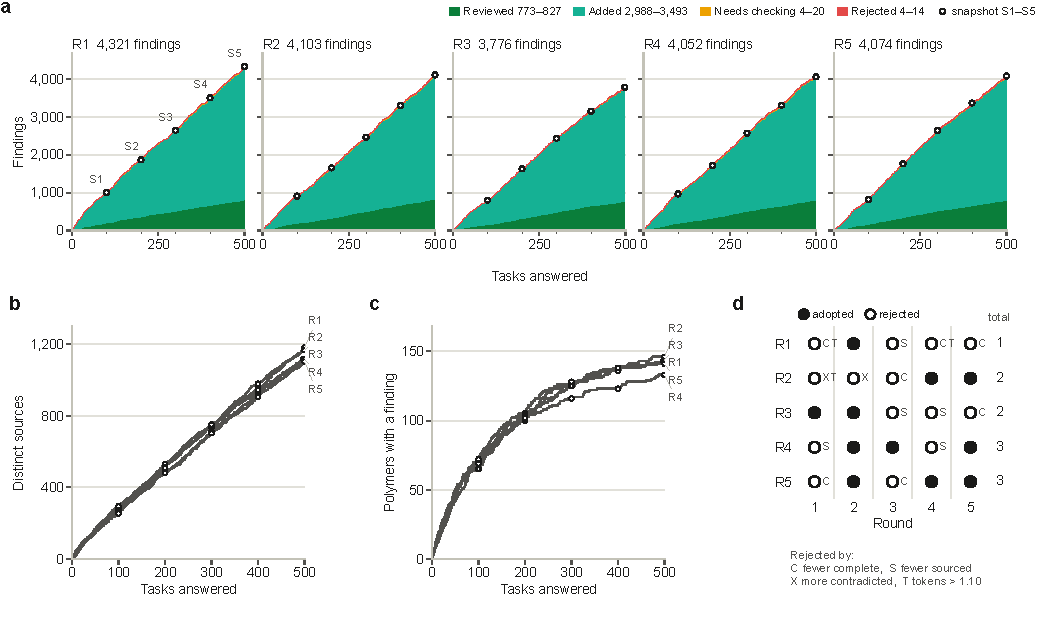
\includegraphics[width=\textwidth]{figures/figS1}
  \caption{The build of the five restarts.
  (a) Findings against tasks answered for each restart, stacked by status (Reviewed, Added, Needs checking, and Rejected, each with its status in the final snapshot), with the snapshots S1--S5 marked.
  (b) Distinct sources against tasks answered, one line per restart.
  (c) Polymers with a finding against tasks answered, one line per restart.
  (d) The improver's proposed edit in each round of each restart, adopted (filled) or rejected (open), with the adoption rules that rejected it: fewer complete answers (C), fewer sourced results (S), more contradicted statements (X), or a token ratio above 1.10 (T).}
  \label{fig:restarts-build}
\end{figure}

\begin{figure}
  \centering
  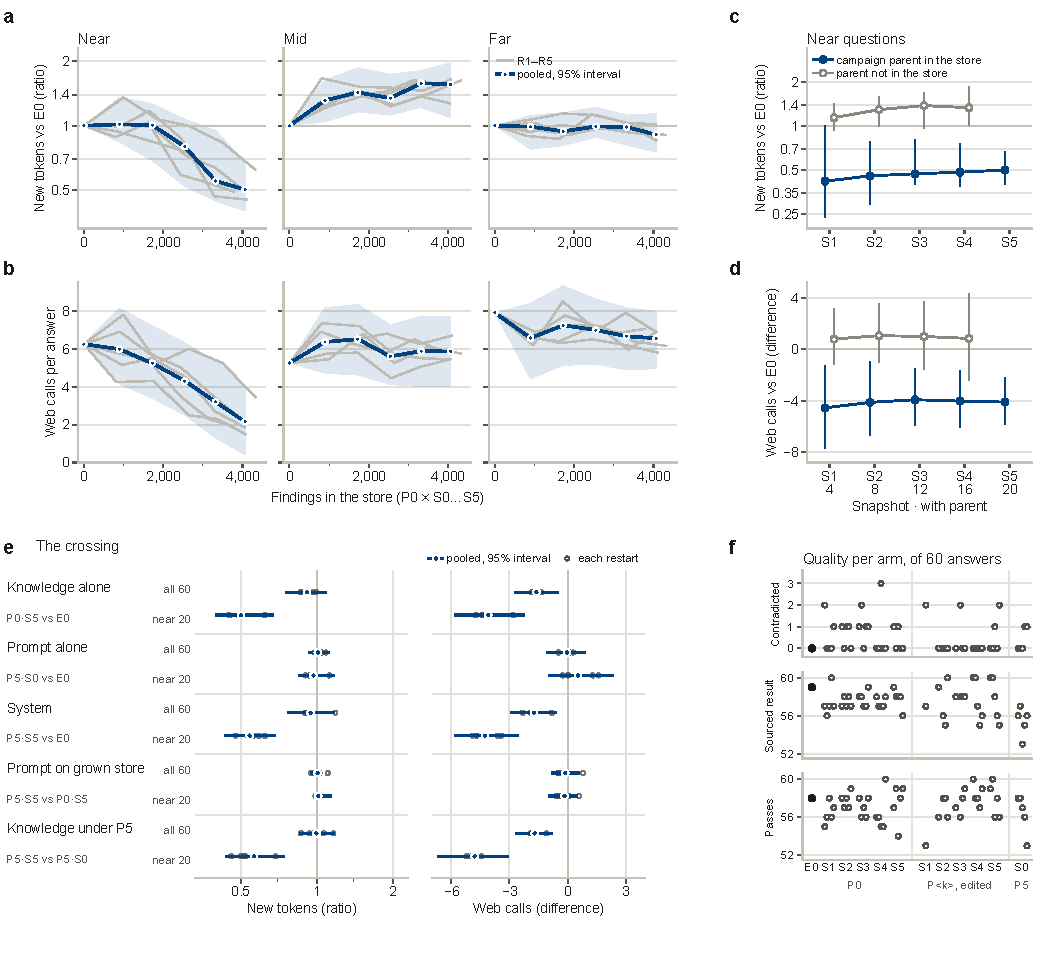
\includegraphics[width=\textwidth]{figures/figS2}
  \caption{The restarts' final evaluation on the 60 held-out questions.
  (a) Knowledge alone: the initial prompt on each snapshot (P0 $\times$ S0--S5) against the empty store (E0), as the median paired new-token ratio by stratum against the findings in the store, one thin line per restart and the pooled estimate with its hierarchical bootstrap 95\% interval.
  (b) The same arms' web calls per answer.
  (c) Near questions on S1--S5, split by whether the question's own campaign parent has a finding in the store: median paired token ratio against E0, pooled over restarts with hierarchical intervals.
  (d) The same split as the difference in web calls per answer, with the number of near questions whose parent is in the store.
  (e) The crossing: knowledge alone (P0S5 against E0), the prompt alone (P5S0 against E0), the system (P5S5 against E0), the prompt on the grown store (P5S5 against P0S5), and the store under the final prompt (P5S5 against P5S0), on all 60 and on the 20 near questions, pooled with hierarchical intervals and per restart.
  (f) Quality per arm: contradicted statements, sourced results, and passes of 60, one dot per arm.}
  \label{fig:restarts-final}
\end{figure}

\subsection{Results}

Five independent restarts from an empty store each built a knowledge base of similar size (Figure~\ref{fig:restarts-build}).
After 500 tasks, the five stores held 3,776 to 4,321 findings, the largest 14.4\% above the smallest, on 133 to 146 polymers, with 2.3\% to 3.9\% of findings lacking a polymer identity.
Every round added 632 to 997 findings, while the number of polymers leveled off, with the first round adding 65 to 72 polymers and the fifth adding three to ten.
Answers citing a saved finding rose in every restart, from 16 to 23 of 100 tasks in the first round to 34 to 46 in the fifth, and revisits cost 0.34 to 0.41 of their parents' tokens.
Reviewers rejected 35 of 4,056 sampled Added findings (0.9\%) and 43 findings in all, most for a material or property label (21) or a method, condition, or scope (9) that the source does not give.
Two of the 2,500 tasks failed for good.

With the initial prompt, each restart's final store cut near-question tokens to 0.45 to 0.62 of the empty store's (pooled 0.50, 0.40--0.67) and near web calls by 2.8 to 4.8 per answer, while far questions stayed flat in four of the five restarts (Figure~\ref{fig:restarts-final}).
Over the five snapshots, the pooled near ratio was 1.01, 1.01, 0.80, 0.55, and 0.50.
The step between the second and fourth snapshots is the near questions' parents arriving, four per round by design.
With the parent's presence in the model, a near question whose parent is in the store costs 0.47 (0.35--0.65) of the baseline, and the store's size adds nothing distinguishable from zero (0.035), as on the resampled stores.
A near question whose parent has not yet been saved costs 1.29 of the baseline, like a mid question.
Variance between restarts is negligible next to this effect (0.0004 on the log scale), and each restart's near slope lies between $-0.32$ and $-0.39$.
The number of findings an answer's searches return saturates at about 22 from the third snapshot onward and is as high for mid questions as for near ones, so it does not predict cost; the parent's presence does.
Contradicted statements did not rise with store size, with 25 in all 3,000 answers, 23 of them in answers that cited no saved finding.

Across the five restarts the improver proposed 25 edits, and the rule adopted 11, one to three per restart.
Four kinds of edit were each adopted in two restarts, namely scoping a claim that a source lacks a detail to the part that was read, answering from the store when its findings cover the question, reopening a cited finding's own source for a missing detail, and repeating knowledge searches less often.
Edits telling the researcher to stop searching the web were proposed five times and adopted once; the other four failed only the guard on sourced results.
In the final evaluation, the final prompts changed cost by nothing measurable, either on the empty store (1.01, 0.93--1.13; web calls 0.0 per answer) or on the grown store (1.01, 0.94--1.04; web calls $-0.1$).
On the empty store they gave a sourced result less often (277 against 295 over the five restarts).
Three arms carrying adopted edits had two contradicted statements where the initial prompt on the same store had none, although over all 24 edited arms the count was 9 against 11.
The saving of about one web call per answer that the recursive test found for its two adopted edits was not reproduced.

%% ---------------------------------------------------------------------------------------------
\section{Ontology Refinement from Answer Traces}
\label{si:ontology}

The ontology refinement (Part~C of the study) asks whether a curator that reads the researcher's traces can change the ontology so that saved knowledge is reached sooner, without making answers worse on withheld questions, and for which questions the ontology matters rather than accumulation.
It holds KF's findings, the prompt (\ident{0b7bb1483235}), and the review policy fixed and changes only the ontology and the annotations of findings.
Each step's inputs were committed by hash before the step that used them, and a second session recomputed every headline number below from the raw records, matching every point estimate (two bootstrap interval ends differed by the random seed only).

\emph{Search changes.}
Two small changes let search read the new kinds of edit, at a new code tag \code{study-freeze-3} (the frozen code plus these only).
The same-source expansion also returns findings from linked sources, and a query's property words also match the names of their property term.
Both do nothing without overlay data: before any run, every recorded search replayed under \code{study-freeze-3} with an empty overlay returned exactly what the frozen code had returned.
All arms ran on \code{study-freeze-3}, the baseline with an empty overlay, so the arms differ only in data.

\emph{Mining.}
The derivation pool is every completed answer with a trace up to 2026-10-21, comprising live-loop answers and the controlled experiments' answers on KF with the web on, excluding the held-out questions: 1,329 answers.
Replaying the recorded searches on KF first had to reproduce their recorded result identifiers exactly.
A miss is one of four events: an answer saved a finding that the duplicate rule matches to one already in KF, and its replayed searches did not return it (saved again); a query, question, or finding's material names a polymer the ontology does not resolve (unresolved name); an answer cited a finding that its first search for that polymer and property did not return (late find); or a search returned nothing and a web search followed for the same polymer and property.
A hop is the run of web searches that leads to one page open, plus the open.
Each hop is classed by what it reached: a source the store did not hold (new knowledge); a source the store held from which the answer took nothing that matches a saved finding (unsaved detail); a source the store did not yet return when the answer ran but KF now returns (reached now); a saved finding that no earlier store search had returned (held but unreached, the most any ontology edit could remove); a page that did not open (failed); a page the answer had already read (repeat); a held source from which the answer took nothing (unused); or web searches that ended without an open (search only).
A store search after the first is classed the same way.
Misses and hops were measured against KF as it is, not the store at the time of the answer, and grouped into a dossier by polymer name, property wording, and candidate source pair, with counts and example trace identifiers.
The pool and KF's stored findings held 750 misses (297 unresolved names, 426 late finds, and 27 saved again): 587 in 230 answers and 163 on stored findings without a polymer identity.

\emph{Edits.}
The edit types form a closed list: a name (a trade name, abbreviation, or spelling of an existing polymer), a polymer (with a broader link to its family, from a reserved block of identifiers), a family link between two existing polymers, an annotation setting or correcting a finding's polymer identity, a source link (a supplement, another version of the same work, a review or data sheet and the primary source it takes a value from, or a paper and the one whose samples or method it reuses), and a property term (a property class with its names and symbols, and the findings annotated to it).
A finding's statement, value, source, and status never change.
A source link stands only on what a source states, such as a supporting information's own heading, Crossref's relation metadata, or a citing passage; that a trace opened two sources one after the other is a reason to look, never evidence of a link.

\emph{Proposal, review, and checks.}
One Claude Code curator session per dossier batch (24 batches) read the dossier, the current ontology records of the polymers involved, and the closed edit list, and proposed edits, each citing the misses or hops it answers; a name or family link carries a source, and a source link quotes the passage or metadata that states the relation.
One fresh Codex reviewer session per batch approved or rejected each edit against its sources with a one-sentence reason.
Deterministic checks then required that no new name map to two unrelated polymers unless marked ambiguous, that family links have no cycles, that every new polymer have a broader link, and that every source link join two sources the store holds.
On the derivation pool only, a replay counted what each edit does: the misses it fixes, the hops it makes reachable, and the results it loses, a result being lost when a finding returned and cited before is no longer returned by the same call.
An edit that loses more results than the misses it fixes and the hops it makes reachable was dropped.
The refined release O is the seed plus the approved overlay, built with the existing release builder, and O, the links overlay, and the annotated store copies were fingerprinted and committed before any withheld question was answered.
The wiki and the pinned seed were not changed.

\emph{Withheld questions.}
Three sets of 60 questions, committed by hash before mining, were withheld from the derivation pool: H, the 60 held-out questions of the controlled experiments; N, new first questions from the campaign generator with a new seed, in the campaign's mix of kinds and never asked word for word before; and L, targeted questions on polymer--property pairs that KF holds with at least three findings, 20 by a name the store does not use, 20 at family level, and 20 asking for a value with its method and specimen.
L was written by one Codex session before mining, from the pairs alone, and the curator never saw it.

\emph{Screen.}
Each withheld question was answered once on three arms: B0 (K0 with the seed ontology), B (KF with the seed ontology), and O+ (KF with the refined ontology), with prompt \ident{0b7bb1483235} and the Codex gpt-6.1-sol researcher on store copies that save nothing; a question's arms were answered in turn and checked together on the same day (540 answers).
B against B0 isolates accumulation, and O+ against B the ontology.
For each question, the accumulation effect $\log(\mathrm{B}/\mathrm{B0})$ and the ontology effect $\log(\mathrm{O{+}}/\mathrm{B})$ were computed for web steps (web calls plus one, so that an answer without a web call counts) and for new tokens.

\emph{Lookup.}
Offline, each withheld question's canonical query (material plus property) and the queries that arm B actually issued were run under both ontologies.
Recall in the first ten results was judged blind by one Codex session per question on the pooled first 25 results of both ontologies, without knowing which returned which; results lost and wrong-polymer results were counted alongside.

\emph{Case studies.}
Because one answer per arm is too noisy to name the questions where the ontology matters, cases were selected by mechanism, from the offline replay and the baseline arm's traces, never from the refined arm's outcome, by a rule committed before the screen.
Each case has three questions drawn from H, N, and L by its rule, with questions written for the purpose where fewer qualified, and each question was answered five times on four arms, B0, O0 (K0 with the refined ontology), B, and O+.
The cases were an unknown name (C1: an approved edit adds a name the seed lacks, and in replay O+ returns relevant findings that B did not), linked sources (C2), a family link (C3), property wording (C4: an approved property term joins the question's wording to the store's), accumulation alone (C5: the seed ontology already returns the relevant findings and the refined ontology changes nothing in replay), nothing saved (C6: KF holds no relevant finding under either ontology), the ontology without knowledge (C7: C1's questions on K0, O0 against B0), and risk (C8: in replay an approved edit brings another polymer's findings into the first ten or pushes a relevant one out).
C2 and C3 were not testable, because no source-link or family-link edit was proposed and approved; the other cases comprised 300 answers, C7 reusing C1's B0 and O0 answers.

\subsection{Results}

\begin{table}
  \caption{The Build of the Refined Ontology, by Edit Type}
  \label{tbl:build}
  \begin{tabular}{lrrrr}
    \toprule
    stage & names & polymer ids & property terms & total \\
    \midrule
    proposed by the curator (24 batches) & 36 & 135 & 26 & 197 \\
    refused by the checks & 2 & 4 & 0 & 6 \\
    approved / rejected by the reviewer & 27 / 7 & 119 / 12 & 17 / 9 & 163 / 28 \\
    unique after assembly & 26 & 114 & 17 & 157 \\
    dropped by the replay & 2 & 4 & 3 & 9 \\
    in force & 24 & 110 & 14 & 148 \\
    \bottomrule
  \end{tabular}
\end{table}

The edits in force comprise 23 distinct names (one was added in two cases), 110 polymer-identity annotations, and 14 property-term edits that make nine terms annotating 649 KF findings (Table~\ref{tbl:build}).
No polymer, family link, or source link was proposed, and the dossier held one candidate source pair.
In sample, on the derivation pool and therefore optimistic, the edits in force fix 197 of the 750 misses (142 unresolved names, 54 late finds, and one saved again), make 31 of the 408 held-but-unreached hops reachable, and lose 40 results.
The drop step caught crowding out, removing two spelling variants of PEEK (losing 21 and 22 results), the tensile-modulus and elongation-at-break terms (31 and 10), a solution-viscosity term, and four annotations.
The reviewer's rejections included blend findings filed under one polymer, names broader than their polymer (``polysulfone'' and ``aliphatic polyketone''), and a glass-transition term that equated the transition with its temperature.

\begin{table}
  \caption{The Withheld Screen (180 Questions per Arm, All Answered and Checked)}
  \label{tbl:screen}
  \small
  \begin{tabular}{lrrrrrrr}
    \toprule
    arm & contradicted & complete & result & passes & citing & web calls & tokens \\
    \midrule
    B0 & 7 & 179 & 161 & 160 & 4 & 6.61 & 48.7k \\
    B & 6 & 174 & 161 & 147 & 101 & 4.41 & 41.7k \\
    O+ & 6 & 175 & 160 & 152 & 96 & 4.26 & 42.2k \\
    \bottomrule
  \end{tabular}
  %% web calls: mean per answer; tokens: median new tokens per answer.
\end{table}

On the withheld screen (Table~\ref{tbl:screen}, in which B0 is K0 with the seed ontology, B is KF with the seed ontology, O+ is KF with the refined ontology, result counts answers giving a sourced result, citing counts answers citing a saved finding, web calls are means, and tokens are medians per answer), O+ against B used 0.99 (0.95--1.02) of the tokens (1.00 on H, 0.99 on N, and 0.98 on L) and 0.97 (0.89--1.06) of the web calls.
B against B0 used 0.88 (0.73--0.99) of the tokens, 0.64 (0.47--0.80) on near, 1.47 on mid, and 1.00 on far questions, and 0.67 (0.56--0.78) of the web calls.
The accumulation effect was the larger in 120 of 180 questions by web steps, the ontology effect in 40 (0.22, 0.16--0.28), and 20 tied; the median ontology ratio was 1.00 against 0.68 for accumulation, and by tokens the split was 132 against 48.

Over all queries, recall in the first ten rose from 0.90 to 0.92 (pooled 0.88 to 0.90), with 84 relevant results gained and 45 lost (2.5\%).
The gain was about equal across the three sets (0.016 on H, 0.015 on N, and 0.017 on L).
The largest gain was on H's mid questions, where pooled recall rose from 0.70 to 0.86 through property terms that reach findings worded otherwise, whereas L's name questions gained nothing (O+ 0.89 against B 0.90), because their trade names never appeared in the traces.
Of B's 373 web hops on the withheld questions, 133 reached new knowledge, 11 an unsaved detail, 16 a source reached now, 1 a held but unreached finding, 185 failed, 3 were repeats, and 24 were searches that ended without an open; B's store searches included 44 held but unreached, and none of these 45 became reachable earlier on O+.

\begin{table}
  \caption{Case Studies of the Ontology Refinement (Three Questions $\times$ Five Replicates per Arm)}
  \label{tbl:cases}
  \begin{tabular}{lcccr}
    \toprule
    & \multicolumn{3}{c}{web calls per answer} & \\
    case & B0 / O0 & B / O+ & & tokens O+/B \\
    \midrule
    C5 accumulation alone & 7.33 / 7.73 & 0.73 / 0.73 & & 1.07 \\
    C4 property wording & 6.20 / 5.87 & 4.07 / 3.33 & & 0.87 \\
    C1 unknown name & 5.60 / 6.00 & 3.33 / 3.40 & & 0.93 \\
    C7 (C1 on K0) & 5.60 / 6.00 & -- & & 0.89 (O0/B0) \\
    C6 nothing saved & 8.00 / 7.80 & 5.20 / 5.53 & & 0.98 \\
    C8 risk in replay & 4.80 / 5.73 & 1.93 / 1.93 & & 1.08 \\
    \bottomrule
  \end{tabular}
\end{table}

In the case studies (Table~\ref{tbl:cases}), knowledge removed about 90\% of web calls where the store covered the topic (C5) and the ontology added nothing there; property wording (C4) showed the largest ontology effect, with a web-call ratio of 0.92; an unknown name (C1) showed about none; where nothing relevant was saved (C6), the refined ontology changed nothing, although KF still cut web calls from 8.00 to 5.20 per answer; and the risk case (C8) showed no visible harm in answers.
The case ratios are medians of per-question ratios over pooled replicates, so a ratio can lie on the other side of 1 from the means.
In C1, B reached the relevant findings by searching other names of the polymer, so the added name changed nothing; C7's O0/B0 ratios (tokens 0.89 and web calls 1.21) lie outside the predicted 0.9 to 1.1 but rest on three questions whose replicates spread across 1 (0.81 to 1.07).

\emph{Predictions.}
All five pre-registered predictions were partly met.
Avoidable hops were at most 15\% of B's web hops, as predicted (1 of 373, in 1 of 180 answers), but most web hops were not limited by accumulation as written, because 185 of the 373 were failed page opens; of the 188 hops that opened a page or ended in a search, 76.6\% reached new knowledge or an unsaved detail, and 85\% did so with the hops reaching a finding saved since.
O+'s recall was at least B's (0.917 against 0.901), but the gain was concentrated in L only on a point estimate, and lost results (2.5\%) exceeded the 2\% limit.
On H and N together, O+ had no more contradicted statements (three against three) and fewer wrong-polymer citations (two against five), but one fewer complete answer (115 against 116) and two fewer results given (110 against 112).
The H and N token ratio lay within 0.9 to 1.1 (1.00, 0.95--1.03), L used fewer web steps on the point estimate only, L did not cite saved findings more often (36 against 37), and C1 showed no effect.
The accumulation effect was the larger for most questions, and C5 and C6 lay within 0.9 to 1.1.
Two records notes apply: C7 is analyzed on all three of C1's questions, as its rule states, although its record labels one, and five verdicts changed when questions answered again after a failed sibling answer were rechecked together, with the analysis using the latest check.

\emph{Limits.}
The refinement was one round by one curator engine, on a base whose topics were already well covered.
The curator could fix only what traces show, so the targeted questions' trade names, which never appeared in the traces, were not added.
Family links are missing from the graph, since family-level questions cited member polymers that the graph does not link to the family, yet no trace surfaced them as misses, so none was proposed.
The approved edits are not yet part of the released seed; adopting them would take a wiki branch and a seed migration, as for the trade names added during the cleanup.

%% ---------------------------------------------------------------------------------------------
\section{Confirmation on the Released Code}
\label{si:confirm}

Parts A and B ran on \code{study-freeze-2}, in which one research session wrote the answer and the findings together, whereas the released code (0.13.0) answers first and writes the findings in a resumed second turn (Section~\ref{si:twoturn}).
A confirmation run checked, on a small pre-registered subset, that the released code reproduces the headline results.
It is not a new study, and Parts A to C stand as recorded.

\emph{Pins.}
The code is tag \code{study-freeze-4} (0.13.0) with researcher prompt \ident{86404bf073ce}; the engines are Codex gpt-6.1-sol for research and checks and Claude Code claude-opus-5-5 for blind case-study scoring.
The stores are KF, read from its frozen copy, and K0; every arm answers on a copy that saves nothing.

\emph{Runs.}
The memory comparison A2 was repeated on two arms, K0 and KF, for the 60 held-out questions in their original order, with one replicate checked together on the same day by one Codex checker (120 answers and checks).
The four case studies were repeated once, as one more replicate of the controlled case studies with the same questions, arms, store copies, and blind scoring (27 answers and their checks).
The measures are those of the controlled experiments, led by contradicted statements, completeness, and sourced results, followed by the new tokens of both turns (comparable with a single session that wrote the same findings), web calls, and time; new for 0.13.0 are the seconds to the answer, the first turn, beside the total.

\emph{Predictions,} committed before any run:
(1) on near questions, the KF/K0 median paired token ratio is at most 0.70 with its interval below 1, and KF makes fewer web calls than K0;
(2) on mid and far questions, each KF/K0 interval includes 1 or, for mid questions, lies above it;
(3) each arm has at most two contradicted statements in its 60 answers, and at most three fewer sourced results than in the comparable controlled replicate;
(4) the case studies go in the same direction as before (the researcher leaves fewer values uncited than the plain session in the first; labels its explanation as interpretation in three of three in the second; ranks more polymers with a sourced value than on an empty store, with fewer tokens, in the third; and no answer gives a value in the fourth); and
(5) KF's median seconds to the answer is below the controlled experiments' median KF seconds for the same questions, which measured the whole single-session answer.
If predictions 1 to 4 hold, the main text describes 0.13.0 and cites this run as evidence that the released code reproduces the results; otherwise it reports \code{study-freeze-2} and says so.

\emph{Results.}
The run took place on 2026-10-27 with every pin holding: all 120 answers of the memory comparison were completed and checked, and the 27 case-study answers were checked and scored blind, with no failed item (Section~\ref{si:accounting}).
All five predictions held (Table~\ref{tbl:confirm}).
The analysis was drawn from the records alone, and its 122 figures agreed with the harness's own reports; a second session recomputed the headline numbers from the answer records without the analysis code.

\begin{table}
  \caption{Confirmation Run on 0.13.0 against the Controlled Experiments on \code{study-freeze-2}}
  \label{tbl:confirm}
  \small
  \begin{tabular}{clll}
    \toprule
    & measure & controlled & confirmation \\
    \midrule
    1 & near, KF/K0 new tokens & 0.52 (0.41--0.57) & 0.60 (0.47--0.63) \\
    1 & near, web calls per answer, K0 / KF & 7.6 / 2.1 & 8.6 / 2.7 \\
    2 & mid, KF/K0 new tokens & 1.29 (0.99--1.52) & 1.14 (0.85--1.41) \\
    2 & far, KF/K0 new tokens & 0.94 (0.82--1.00) & 0.89 (0.71--1.37) \\
    3 & contradicted statements, K0 / KF & 0 / 1 in 180 & 1 / 0 in 60 \\
    3 & sourced results, K0 / KF & 58.0 / 57.0 of 60\textsuperscript{\emph{a}} & 55 / 57 of 60 \\
    4 & cs1, uncited Tg values, R / P & 1--13 / 14--33 & 9 / 31 \\
    4 & cs2, explanation labelled, R & 3 of 3 & 3 of 3 \\
    4 & cs3, ranked with sourced value, R / R0 & 8--9 / 3--5 & 8 / 4 \\
    4 & cs3, new tokens, R / R0 & 117k--155k / 145k--213k & 117.1k / 180.5k \\
    4 & cs4, value given as reported & 0 of 9 & 0 of 9 \\
    5 & KF, median seconds to the answer & 66.6\textsuperscript{\emph{b}} & 40.5 \\
    \bottomrule
  \end{tabular}

  The first column gives the prediction. \textsuperscript{\emph{a}} Mean per replicate of three. Ranges for the case studies are over five replicates. \textsuperscript{\emph{b}} The whole single-session answer.
\end{table}

\emph{Quality.}
K0's one contradicted statement, on a mid question, cited the wrong section of the right source; KF had none.
K0's 55 sourced results lay exactly at the limit of prediction 3, three below the controlled mean of 58.0 per replicate (57 to 59), and KF's 57 lay within its controlled range (56 to 58).
All of K0's answers and 59 of KF's were complete, and 53 and 55 answers passed.
The checker marked access as uncertain in 10 answers per arm, against 4 and 22 in the controlled experiment's 180.
In the case studies, one R answer in cs2 and one P answer in cs3 had a contradicted statement, as in one and four of the earlier five replicates.

\emph{Cost and time.}
Paired per question against the controlled experiment's three replicates of the same arm, the released code used 1.26 (1.17--1.42) times the new tokens on K0 and 1.27 (1.10--1.48) on KF.
Its median new tokens per answer, 53.1k on K0 and 44.8k on KF, lie above the controlled replicates' medians (41.3k to 44.4k and 33.9k to 39.7k).
The second turn accounts for 12.9\% of K0's new tokens and 11.3\% of KF's (medians 6.2k and 5.4k per answer), and web calls rose from 6.9 to 7.6 per answer on K0 and from 4.5 to 5.2 on KF.
The answer turn on K0 alone (median 47.1k) therefore cost more than the controlled single session, which also wrote the findings.
With one replicate, we cannot attribute that remainder to the split or to the day; the eight-question parity set had shown the opposite direction (Section~\ref{si:twoturn}).
In the case studies, the researcher's new tokens lay within the earlier five replicates' range in four of its six arms, just below it for R in cs3 (117.1k against 117.4k to 154.9k), and above it for R in cs1 (190k against 112k to 167k); the plain session's lay above its range only in cs2 (444k against 288k to 336k, with 52 web calls).
The answer arrived sooner: on KF after a median 40.5~s, 0.75 (0.69--0.85) of the controlled single session's time on the same questions, and on K0 after 56.6~s against 80.7~s.
Writing the findings took a further median 48.3~s on KF, so the total time was 1.30 (1.18--1.51) times the single session's.
Of the 120 second turns, 119 read at least 82\% of their input from the prompt cache (median 96\%); in the remaining one, the first answer of the run, the cache missed entirely and the second turn cost 69k new tokens.
Seconds depend on how many sessions run at once, which differed between the runs.

%% ---------------------------------------------------------------------------------------------
\section{Records Analyses}
\label{si:records}

The knowledge base was characterized from its records without further engine calls.
Each finding's property string was assigned to one of 183 property classes, 143 of them material properties in 18 categories, by stored manual assignments and ordered rules, with the remainder classified in one model pass.
A second, blind classification of 600 strings, the 300 most frequent and 300 drawn at random, agreed with the map for 94\% of strings, covering 98.5\% of the findings they label.
Because both classifiers are language models, this measures consistency rather than agreement with an expert.
For the glass transition temperature analysis, a finding's method was read from its property string, or else from its conditions but never from its statement.
DSC includes temperature-modulated DSC and the DSC test standards, DMA includes dynamic mechanical spectroscopy, the tan~$\delta$ peak, and the DMA standards, and only findings with a single readable temperature were kept.
Source metadata (type, publisher, year, and open-access indication) were obtained from Crossref by DOI; only DOIs left the machine.
Reuse was computed from the recorded tool payloads, with a finding counted as returned when it appeared in a later session's search result and as cited when a later answer cited its identifier.

%% ---------------------------------------------------------------------------------------------
\section{Statistics}
\label{si:stats}

All comparisons between arms are paired by question.
Each arm's replicates of a question are pooled by the geometric mean of their new tokens, and an arm's cost relative to another is reported as the median over questions of the paired token ratio, with a bootstrap 95\% interval over questions (2,000 resamples).
Web-call differences are reported as the mean paired difference with the same interval.
The dependence of cost on store size is estimated as the slope of log new tokens on log store findings with a fixed effect for each question, one slope per stratum.
For the resampled stores, a second model adds an indicator for whether the campaign question from which a near question was drawn is present in the store, which separates topic coverage from store size.
The dependence of passing on store size is estimated by mixed logistic regression with a fixed effect for stratum and a random intercept for each question, fit by variational Bayes in statsmodels.\cite{Seabold2010Statsmodels}
A generalized estimating equation fit with robust intervals was used as a sensitivity check on this model.
For the restarts, intervals come from a hierarchical bootstrap over restarts and then questions, and the scaling slope from a mixed model with random effects for question and restart.
The rules for calling a restart effect flat, smaller, or raised were written into the analysis code before any final number was computed.
For the ontology refinement, shares of questions and the web-call ratio come with the same bootstrap interval over questions, and case ratios are medians of per-question ratios over pooled replicates.
With 60 held-out questions, only large effects are detectable; smaller differences are reported as estimates with their intervals.
All analyses are descriptive, and no result gated another.

%% ---------------------------------------------------------------------------------------------
\section{Run Accounting}
\label{si:accounting}

Across the controlled experiments and the restarts, 10,418 answers and 8,220 checks were completed in 20,572 engine sessions (20,473 on Codex and 99 on Claude Code), using 703.5 million new tokens.
Of these sessions, 179 failed with a named reason (85 timeouts, 32 crashes, 18 interruptions, 3 rate limits, and 41 sessions that the machine slept through); 176 of them were retried and completed, and three, two of them restart tasks, failed for good.
The ontology refinement ran 24 curator and 24 reviewer sessions, one session writing the targeted questions, 180 blind relevance judgments, 540 screen answers, and 300 case-study answers, each with its check, and none of the screen's answers failed.
The confirmation run completed 294 Codex sessions, 240 for the memory comparison (120 two-turn answers and 120 checks) and 54 for the case studies (27 answers, 16 of them in two turns, and 27 checks), and four Claude Code sessions for blind scoring, with about 13.2 million new tokens on Codex; one check timed out and was retried, and no item failed.

%% ---------------------------------------------------------------------------------------------
\section{The Researcher's Prompt}
\label{si:prompts}

The frozen prompt \ident{0b7bb1483235}, used by every experiment except the confirmation run, is reproduced below; the question is appended after it.

\lstinputlisting{si/prompt-0b7bb1483235.txt}

The released code (0.13.0) splits the prompt into the answer turn and the deposit turn, identified together by \ident{86404bf073ce}; their rules were moved verbatim.

\emph{Answer turn.}
\lstinputlisting{si/prompt-86404bf073ce-answer.txt}

\emph{Deposit turn.}
\lstinputlisting{si/prompt-86404bf073ce-deposit.txt}

\bibliography{refs}

\end{document}
